\begin{figure}[h]
  \centering
  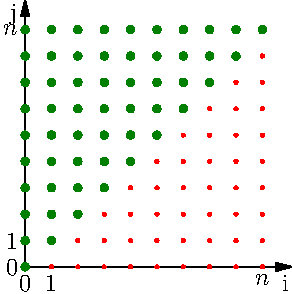
\includegraphics{./Csomm5_1.pdf}
  % Csomm5_1.pdf: 0x0 pixel, 0dpi, 0.00x0.00 cm, bb=
  \caption{Domaine de sommation triangulaire au dessus de la diagonale}
  \label{fig:Csomm5_1}
\end{figure}
\begin{enumerate}
  \item 
  \begin{enumerate}
    \item Le domaine de sommation est formé par les couples $(i,j)$ tels que $i\leq j$. Il est représenté sur la figure \ref{fig:Csomm5_1} par les points du triangle au dessus de la diagonale. Dans l'expression de $S$, on somme d'abord sur les colonnes avant d'additionner ces sommes intermédiaires.
    \item Quand on intervertit les sommations, on somme d'abord sur les lignes ce qui permet d'utiliser la formule du binôme:
\begin{displaymath}
S = \sum_{j=1}^{n}\sum_{i=0}^{j}\binom{j}{i}\binom{n}{j}  
= \sum_{j=1}^{n}\left( \binom{n}{j}\sum_{i=0}^{j}\binom{j}{i}\right) 
= \sum_{j=1}^{n}\binom{n}{j}2^j = 3^n
\end{displaymath}
  \end{enumerate}

  \item On trouve $s(1,n)=2^n$ et $s(2,n)=3^n$ car
\begin{displaymath}
  s(1,n) = \sum_{i=0}^n\binom{n}{i}\;\text{ et } s(2,n) = S = 3^n
\end{displaymath}

\item
\begin{enumerate}
  \item En réécrivant $M(1,n)$, une formule du binôme apparait:
\begin{displaymath}
M(1,n) = \sum_{i_1=0}^{n}\binom{n}{i_1}a_0^{i_1}a_1^{n-i_1} = (a_0 + a_1)^n  
\end{displaymath}
Montrons que pour $k\leq p$,
\begin{displaymath}
  M(k-1,n)=(a_0 + \cdots + a_{k-1})^n \Rightarrow M(k,n)=(a_0 + \cdots + a_{k-1} + a_k)^n
\end{displaymath}
En effet, $M(k,n)$ s'écrit 
\begin{multline*}
\sum_{i_k=0}^{n}
\left( 
\sum_{ 0\leq i_1 \leq \cdots \leq i_{k-1} \leq i_k}
\binom{i_2}{i_1}\binom{i_3}{i_2}\cdots \binom{i_k}{i_{k-1}}
a_0^{i_1}a_1^{i_2-i_1}\cdots a_{k-1}^{i_k - i_{k-1}}
\right)
\binom{n}{i_k}a_k^{n-i_k} \\
= \sum_{i_k=0}^{n} M(k-1,n)\binom{n}{i_k}a_k^{n-k} 
= \sum_{i_k=0}^{n} (a_0+\cdots+a_{k-1})^{i_k}\binom{n}{i_k}a_k^{n-k}\\
= (a_0 + \cdots + a_{k})^n
\end{multline*}

  \item Utilisons l'expression d'un coeficient du binôme ne contenant que des factorielles:
\begin{displaymath}
  \binom{q}{p} = \frac{q!}{p!(q-p)!}
\end{displaymath}
Les $j_k$ s'introduisent naturellement et des simplifications (télescopiques multiplicatives) apparaissent dans le produit des coefficients
\begin{displaymath}
  \binom{i_2}{i_1}\binom{i_3}{i_2}\cdots \binom{i_p}{i_{p-1}}\binom{n}{i_p}
= \frac{i_2!}{i_1!j_2!} \frac{i_3!}{i_2!j_3!} \cdots \frac{i_p!}{i_{p-1}!j_p!} \frac{n!}{i_p!j_p!} 
= \frac{n!}{j_1!\, j_2!\, \cdots \, j_p!}
\end{displaymath}
car $i_1 = j_1$.
\end{enumerate}

\end{enumerate}
